\documentclass[border=6pt]{standalone}
\usepackage[T1]{fontenc}
\usepackage[utf8]{inputenc}
\usepackage[scaled=0.98]{helvet}
\renewcommand{\familydefault}{\sfdefault}
\usepackage{amsmath}
\usepackage{graphicx}
\graphicspath{{../../../../../../exercises_lecturenotes/lecture_notes/kurs100_lektionsnoter/}}
\usepackage{tikz}
\usepackage{pgfplots}
\pgfplotsset{compat=1.18}
\usetikzlibrary{arrows.meta, decorations.pathreplacing, calc, positioning, fit, backgrounds, shapes.geometric}
\usepgfplotslibrary{groupplots,fillbetween}
\definecolor{scanpink}{HTML}{E5006D}
\definecolor{scanteal}{HTML}{00A6A6}
\definecolor{scannavy}{HTML}{243746}
\definecolor{scanlightgray}{HTML}{F1F2F3}
\begin{document}
  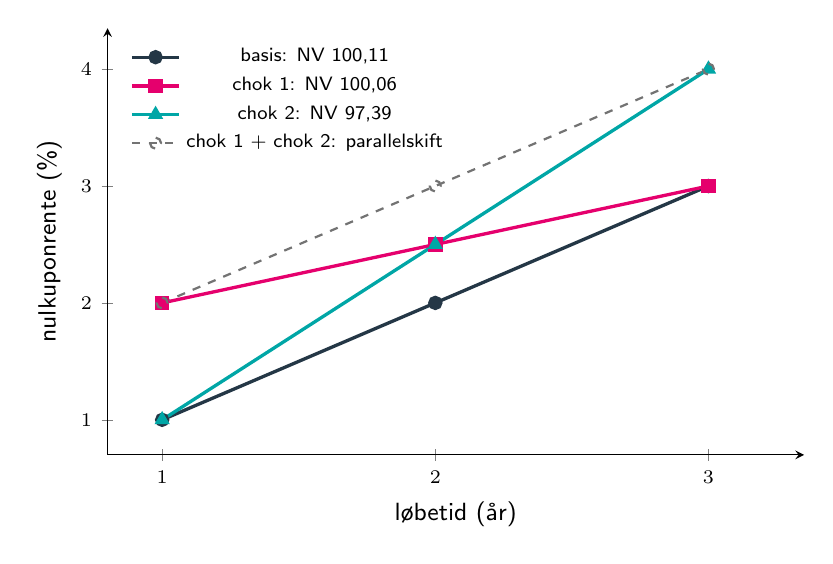
\begin{tikzpicture}
    \begin{axis}[
      width=0.86\textwidth,
      height=7.0cm,
      axis lines=left,
      xlabel={løbetid (år)},
      ylabel={nulkuponrente (\%)},
      xmin=0.8, xmax=3.35,
      ymin=0.7, ymax=4.35,
      xtick={1,2,3},
      ytick={1,2,3,4},
      legend style={draw=none, fill=none, font=\scriptsize, at={(0.02,0.98)}, anchor=north west},
      tick label style={font=\scriptsize},
      label style={font=\small}
    ]
      \addplot[scannavy, very thick, mark=*] coordinates {(1,1) (2,2) (3,3)};
      \addlegendentry{basis: NV 100,11}
      \addplot[scanpink, very thick, mark=square*] coordinates {(1,2) (2,2.5) (3,3)};
      \addlegendentry{chok 1: NV 100,06}
      \addplot[scanteal, very thick, mark=triangle*] coordinates {(1,1) (2,2.5) (3,4)};
      \addlegendentry{chok 2: NV 97,39}
      \addplot[black!55, thick, dashed, mark=o] coordinates {(1,2) (2,3) (3,4)};
      \addlegendentry{chok 1 + chok 2: parallelskift}
    \end{axis}
  \end{tikzpicture}
\end{document}
